\section{Forcing as strict extension}\label{sec:forcing}

The Six Birds framework proves, in its finite setting, a counting lemma about how rarely a random
predicate is definable from a coarse partition. It was called, half in jest, the ``finite forcing
lemma''~\citep{SBTFoundationsI}, with an explicit warning that its kinship with Cohen's forcing
\citep{Cohen1963,Cohen1966} was only an analogy. This section makes the kinship precise and marks
where it stops.

The finite lemma counts the failures of the same \emph{disagreement} and \emph{splitting}
conditions that Cohen forcing uses (\S\ref{ssec:finitebridge}). Over $\omega$ those failures
disappear (\S\ref{ssec:vanish}), and as a consequence a Cohen-generic real over a countable
transitive model is new, splits every infinite set the model can code, and strictly enlarges the
algebra of predicates the model can express (\S\S\ref{ssec:genericity}--\ref{ssec:strict}). The
implication runs in one direction only. Novelty and splitting do not make a real generic; we give
an explicit counterexample and the exact test that does characterize genericity
(\S\ref{ssec:converse}). Finally, the finite probabilities measure novelty, not genericity:
Cohen reals form a set that is large in the sense of category but has measure zero
(\S\ref{ssec:category}).

\subsection{The finite Cohen bridge}\label{ssec:finitebridge}

Fix a finite index set $Z$ of size $N$ and a lens $f\colon Z\to X$ with $K$ nonempty blocks
$B_x=f^{-1}(x)$; the degenerate case $N=K=0$ is allowed. A \emph{predicate} is a total map
$h\colon Z\to\{0,1\}$. It is \emph{definable from $f$}, or visible to $f$, if it is constant on
every block. This is the paper's observational convention, not formula definability in a
specified language \citep[for which see][]{Libkin2004}. Equivalently, $h$ is definable from $f$
if the refined lens $z\mapsto(f(z),h(z))$ induces the same partition as $f$.

The \emph{finite Cohen poset} $\Cgen_Z$ consists of the partial functions $p\colon
Z\rightharpoonup\{0,1\}$, with $q\le p$ when $q$ extends $p$. A total predicate $h$ determines the
\emph{restriction filter} $G_h=\{p:p\subseteq h\}$. For a definable $g$, and for a block $B_x$ with
at least two elements, consider
\[
\begin{aligned}
  D_g&=\{p:\ p(z)\ne g(z)\text{ for some }z\in\dom p\},\\
  E_x&=\{p:\ p(z)\ne p(z')\text{ for some }z,z'\in B_x\cap\dom p\}.
\end{aligned}
\]

\begin{lemma}[Meeting equivalences; \inhouse]\label{lem:meeting}
For every total $h$:
\begin{enumerate}\itemsep0pt
\item $G_h$ meets $D_g$ iff $h\ne g$. Hence $h$ is not definable from $f$ iff $G_h$ meets $D_g$
for every definable $g$.
\item $G_h$ meets $E_x$ iff $h$ is not constant on $B_x$. Hence $h$ splits every block with at
least two elements iff $G_h$ meets every $E_x$.
\end{enumerate}
\end{lemma}

The two conditions in the lemma are different. A non-definable $h$ need only split \emph{some}
block; splitting \emph{every} non-singleton block is stronger.

\begin{theorem}[Density defects; \inhouse]\label{thm:densitydefect}
For a family $\mathcal D$ of conditions, let $F(\mathcal D)=\{p:\text{no }q\le p\text{ lies in
}\mathcal D\}$ be the set of conditions that have no extension in $\mathcal D$. Then
\[
  F(D_g)=\{g\},\qquad
  F(E_x)=\{p:\ B_x\subseteq\dom p\text{ and }p\restr B_x\text{ is constant}\}.
\]
So the only condition with no extension in $D_g$ is the total condition $g$ itself, and the
conditions with no extension in $E_x$ are exactly those that have already fixed the whole block to
a constant.
\end{theorem}

\begin{proof}
For $D_g$: a condition that is not a restriction of $g$ already disagrees with $g$ somewhere, so
it lies in $D_g$. A proper restriction of $g$ leaves some coordinate $z$ free, and setting it to
$1-g(z)$ gives an extension in $D_g$. The total condition $g$ has no extension but itself, which
is not in $D_g$. For $E_x$: if $p$ fixes $B_x$ to a constant, no extension splits the block.
Otherwise, either $p$ already splits $B_x$; or $p$ assigns at least one bit on $B_x$ and leaves
another coordinate of $B_x$ free, which can be set to the opposite value; or $p$ assigns no bit on
$B_x$, and two free coordinates of $B_x$ can be set to $0$ and $1$.
\end{proof}

\begin{remark}[Genericity in the finite poset is trivial]\label{rem:finitegeneric}
In $\Cgen_Z$ a total condition has no proper extension, so a genuinely dense family contains
every total condition, and every restriction filter $G_h$ meets every dense family. The families
$D_g$ are not dense: $g$ has no extension in $D_g$. The finite statements in this subsection are therefore about meeting
these particular \emph{defective} families, not about genericity in the finite poset.
\end{remark}

\begin{theorem}[The counting lemma; \inhouse]\label{thm:counting}
Let $h$ be a uniformly random total predicate. Then
\begin{enumerate}\itemsep0pt
\item $h$ is definable from $f$, equivalently $G_h$ misses some $D_g$, with probability exactly
$2^{-(N-K)}$;
\item $h$ splits every block with at least two elements, equivalently $G_h$ meets every $E_x$, with
probability exactly $\prod_{|B_x|\ge2}\bigl(1-2^{1-|B_x|}\bigr)$, and hence with probability at
least $1-\sum_{|B_x|\ge2}2^{1-|B_x|}$.
\end{enumerate}
\end{theorem}

\begin{proof}
(1) By Lemma~\ref{lem:meeting}, $G_h$ misses $D_g$ exactly when $h=g$. There are $2^K$ definable
predicates, one bit per block, among $2^N$ predicates in all, giving $2^K/2^N$. (2) The blocks are
disjoint, so the events ``$h$ is constant on $B_x$'' are independent, each with probability
$2\cdot2^{-|B_x|}$. The product and the union bound follow.
\end{proof}

When $K=N$ every block is a singleton: every predicate is definable, and splitting every
non-singleton block holds vacuously. Theorem~\ref{thm:counting}(1) \emph{is} the framework's
finite forcing lemma. Its rarity $2^{-(N-K)}$ is the probability that $h$ lands exactly on the
defect $F(D_g)=\{g\}$ of one of the disagreement families. The lemma is therefore the statistics of
the density families that forcing uses, at a finite size where those families are defective.

\subsection{Over \texorpdfstring{$\omega$}{omega} the defects vanish}\label{ssec:vanish}

Let $\Cgen=\Fn(\omega,2)$ be the poset of finite partial functions $p\colon\omega
\rightharpoonup\{0,1\}$, ordered by extension: the finite Cohen poset over the infinite index
$\omega$. Define $D_g$ for any total $g\colon\omega\to\{0,1\}$, and $E_A$ for any $A\subseteq\omega$,
exactly as above.

\begin{corollary}[Infinite-index contrast; \inhouse]\label{cor:infinitecontrast}
In $\Fn(\omega,2)$, $D_g$ is dense for every total $g$, and $E_A$ is dense for every
\emph{infinite} $A\subseteq\omega$. A finite $A$ with at least two elements keeps its defect.
\end{corollary}

\begin{proof}
A finite condition leaves infinitely many coordinates free. One of them can be set against $g$,
and an infinite $A$ contains two free coordinates, which can be set to $0$ and $1$. A condition
that fixes a finite $A$ to a constant has no extension splitting $A$.
\end{proof}

The finite defect $\{g\}$ disappears because no finite condition is total over $\omega$, and the
splitting defect disappears because no finite condition fixes an infinite block. What was rare in
the finite count becomes dense, and density is what genericity meets.

\subsection{Generic reals are new}\label{ssec:genericity}

We use two named hypotheses.
\begin{description}[leftmargin=1.2em]
\item[\textbf{J1}.] There is a countable transitive model $M$ of $\mathsf{ZFC}$. Its countability
is external: inside $M$, the set of reals is uncountable.
\item[\textbf{J2}.] The classical generic-extension machinery \citep{Cohen1966,Kunen2011}: if $G$
is $\Cgen$-generic over $M$, there is a transitive model $M[G]$ of $\mathsf{ZFC}$ with
$M\subseteq M[G]$, $G\in M[G]$, and the same ordinals as $M$.
\end{description}
The results of this subsection and the next use \textbf{J1} only; \textbf{J2} is used only to name
the model in which the new real lives.

\begin{definition}[Coded predicates]\label{def:groundlens}
Let $\mathcal B_M:=\powset(\omega)\cap M$, the subsets of $\omega$ that belong to $M$; we identify
each with its characteristic function, an \emph{$M$-coded predicate} on $\omega$. Since $M$ is a
transitive model, $\mathcal B_M$ contains $\varnothing$ and $\omega$ and is closed under finite
Boolean operations; it is a Boolean algebra of predicates on $\omega$.
\end{definition}

\begin{lemma}[Few coded predicates; \condg, under \textbf{J1}]\label{lem:countable}
$\mathcal B_M$ is countable, while $2^\omega$ is uncountable.
\end{lemma}

This is the infinitary counterpart of $2^K$ visible predicates among $2^N$. The analogy has a
limit, discussed in \S\ref{ssec:strict}: $\mathcal B_M$ is not the family of predicates visible to
any partition of $\omega$.

\begin{lemma}[Generics exist; \condg, under \textbf{J1}]\label{lem:RS}
For every $p\in\Cgen$ there is a filter $G\ni p$ that meets every dense subset of $\Cgen$ lying in
$M$.
\end{lemma}

\begin{proof}
Since $M$ is transitive and computes $\omega$ correctly, the poset $\Cgen$ as computed in $M$ is
the actual poset, and density of a set in $M$ means the same inside $M$ as outside. Because $M$ is
countable, enumerate its dense subsets of $\Cgen$ as $D_0,D_1,\dots$ and fix an enumeration of
$\Cgen$. Build $p=p_0\ge p_1\ge\cdots$, with $p_{n+1}$ the first extension of $p_n$ in $D_n$ in that
enumeration, so that no choice principle is used. The upward closure of the chain is a filter
containing $p$ and meeting every $D_n$. This is the Rasiowa--Sikorski lemma
\citep{RasiowaSikorski1950}.
\end{proof}

\begin{theorem}[Generic reals are new; \condg, under \textbf{J1}]\label{thm:novelty}
Let $G$ be $\Cgen$-generic over $M$ and $x_G:=\bigcup G$. Then $x_G\colon\omega\to\{0,1\}$ is
total, $G$ is exactly the restriction filter $\{p:p\subseteq x_G\}$, and:
\begin{enumerate}\itemsep0pt
\item $x_G\ne y$ for every $y\in\mathcal B_M$; in particular $x_G\notin M$;
\item $x_G$ splits every infinite $A\in\mathcal B_M$: there are $m,n\in A$ with $x_G(m)\ne x_G(n)$.
\end{enumerate}
\end{theorem}

\begin{proof}
Conditions in a filter are compatible, so $x_G$ is a function. The sets $T_n=\{p:n\in\dom p\}$ are
dense and lie in $M$, so $G$ meets each of them and $x_G$ is total. Every $p\in G$ is a
restriction of $x_G$; conversely, a finite restriction of $x_G$ is contained in a common extension
of finitely many members of $G$, which lies in $G$, so it lies in $G$ by upward closure. For (1),
let $y\in\mathcal B_M$. The family $D_y$ is dense (Corollary~\ref{cor:infinitecontrast}) and lies in
$M$, being defined there from $y$. So $G$ meets $D_y$, and $x_G$ disagrees with $y$ somewhere. Every
real in $M$ is such a $y$, so $x_G\notin M$. For (2), let $A\in M$ be infinite. Then $E_A$ is dense
(Corollary~\ref{cor:infinitecontrast}) and lies in $M$, so $G$ meets it.
\end{proof}

The generic real thus escapes the ground model through the same disagreement families $D_y$ that
appear in the finite lemma, now dense because the index set is infinite.

\subsection{Novelty is not genericity}\label{ssec:converse}

The finite lemma suggests a converse: perhaps a real that is new and splits every infinite coded
set is already generic. It is not.

\begin{proposition}[The converse fails; \condg, under \textbf{J1}]\label{prop:converse}
There is a total $x\colon\omega\to\{0,1\}$ such that $x\notin M$ and $x$ splits every infinite
$A\in\mathcal B_M$, but the restriction filter of $x$ is not generic over $M$.
\end{proposition}

\begin{proof}
By Lemma~\ref{lem:RS} take a generic $G$ and let $r=x_G$. Define the \emph{duplicated} real
$x(2n)=x(2n+1)=r(n)$. If $x$ were in $M$, so would be $r(n)=x(2n)$; hence $x\notin M$. Let $A\in M$
be infinite, and let $B=\{\lfloor a/2\rfloor:a\in A\}$. Then $B\in M$, and $B$ is infinite, since the
preimage of a finite $B$ would have at most $2|B|$ elements. By Theorem~\ref{thm:novelty}(2), $r$
splits $B$: there are $b,b'\in B$ with $r(b)\ne r(b')$. Choosing $a,a'\in A$ with $\lfloor
a/2\rfloor=b$ and $\lfloor a'/2\rfloor=b'$ gives $x(a)=r(b)\ne r(b')=x(a')$, so $x$ splits $A$.
Now consider
\[
  D^\ast=\{p:\ \text{for some }n,\ 2n,2n+1\in\dom p\text{ and }p(2n)\ne p(2n+1)\}.
\]
$D^\ast$ is defined without parameters, so it lies in $M$, and it is dense: above any condition,
choose a pair $2n,2n+1$ beyond its domain and assign $0$ and $1$. No restriction of $x$ lies in
$D^\ast$, so the restriction filter of $x$ misses a dense set in $M$.
\end{proof}

Genericity therefore asks for more than novelty and splitting. The exact requirement is meeting
\emph{every} dense set coded in $M$, and it has a clean topological form. Give $2^\omega$ the
product topology, whose basic open sets are the cylinders $[p]=\{x: p\subseteq x\}$. A \emph{tree} is a
set $T$ of conditions closed under restriction. A closed set $F\subseteq2^\omega$ is \emph{coded in
$M$} if $F=[T]$ for a tree $T\in M$, where $x\in[T]$ iff every finite restriction of $x$ lies in
$T$. The code is in $M$; its branches are computed outside $M$ and may include reals that are not
in $M$. Because the tree is finitely branching, emptiness of $[p]\cap[T]$ is decided at a finite
level:
\[
  [p]\cap[T]=\varnothing\iff\exists n\ \bigl(\dom p\subseteq n\ \wedge\ \forall s\in2^n\
  (p\subseteq s\Rightarrow s\notin T)\bigr).
\]
This criterion is arithmetic in $p$ and $T$, hence absolute for the transitive model $M$, and so
are the statements that $[T]$ is nowhere dense and that a family of conditions in $M$ is dense
(since $M$ contains exactly the actual finite conditions).

\begin{theorem}[Exact recognition of genericity; \condg, under \textbf{J1}]\label{thm:recognition}
For a total $x\colon\omega\to\{0,1\}$, the restriction filter $G_x=\{p:p\subseteq x\}$ is generic
over $M$ if and only if $x$ lies in no closed nowhere dense subset of $2^\omega$ coded in $M$.
\end{theorem}

\begin{proof}
($\Rightarrow$) Let $F=[T]$ be closed nowhere dense with $T\in M$. By the arithmetic criterion
above and Separation in $M$, the conditions $p$ with $[p]\cap F=\varnothing$ form a family in $M$,
and it is dense because $F$ is nowhere dense. A
generic $G_x$ meets it, so some $p\subseteq x$ has $[p]\cap F=\varnothing$, and $x\notin F$.
($\Leftarrow$) Let $D\in M$ be dense. Let $T_D$ be the set of conditions none of whose restrictions
lies in $D$; it is a tree, and it belongs to $M$ by Separation from $D$; and its branch set $F_D=[T_D]$ is the complement of the open set
$\bigcup_{p\in D}[p]$. Density of $D$ makes that open set dense, so $F_D$ is closed nowhere dense
and coded in $M$. If $x\notin F_D$, some restriction of $x$ lies in $D$, so $G_x$ meets $D$.
\end{proof}

The tests used in Theorem~\ref{thm:novelty} are special cases: avoiding the singleton $\{y\}$ for
$y\in M$ is meeting $D_y$, and avoiding the closed set of reals constant on an infinite $A\in M$ is
meeting $E_A$. They form a proper subfamily of all coded closed nowhere dense tests. The
duplicated real of Proposition~\ref{prop:converse} passes all of them and fails the test
belonging to $D^\ast$: it lies in the coded closed nowhere dense set of reals that are constant on
every pair $\{2n,2n+1\}$. Figure~\ref{fig:genericity} summarizes the relations. The density of
$D^\ast$, the fact that every duplicated real misses it, and the construction of the obstruction
trees $T_D$ with their nowhere density are verified in Lean (\S\ref{sec:mech}); the existence of $M$
and of generic reals is not.

\begin{figure}[tbp]
\centering
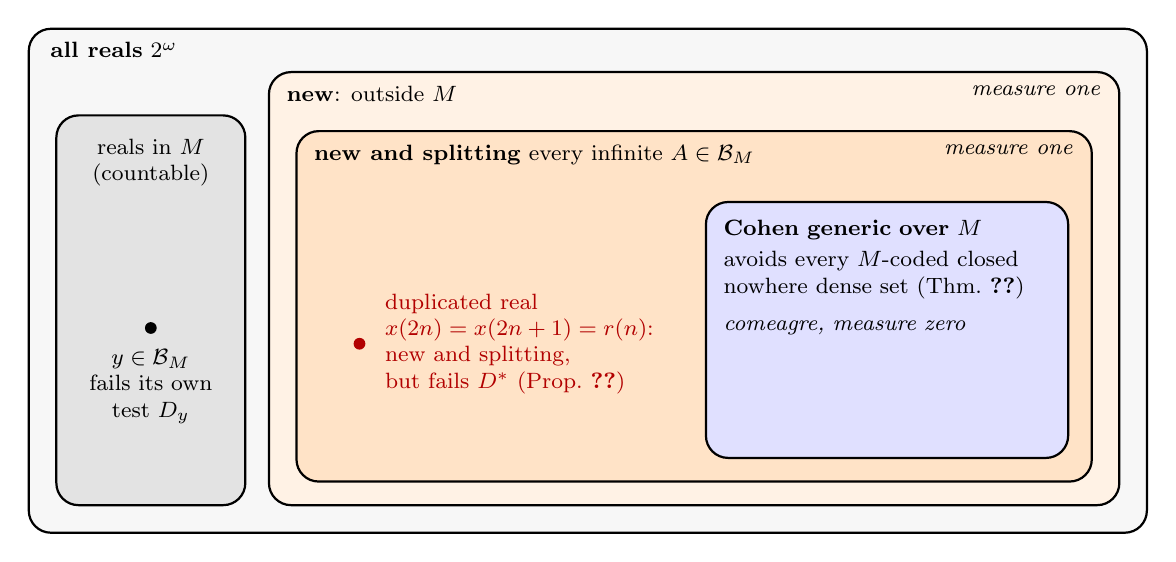
\begin{tikzpicture}[
    font=\footnotesize,
    reg/.style={draw, rounded corners=8pt, thick},
    dot/.style={circle, fill, inner sep=1.5pt}]
  % all reals
  \draw[reg, fill=gray!6] (0,0) rectangle (14.2,6.4);
  \node[anchor=north west] at (0.15,6.35) {\textbf{all reals} $2^\omega$};
  % reals in M
  \draw[reg, fill=gray!22] (0.35,0.35) rectangle (2.75,5.3);
  \node[align=center] at (1.55,4.7) {reals in $M$\\(countable)};
  \node[dot] at (1.55,2.6) {};
  \node[anchor=north, align=center] at (1.55,2.45) {$y\in\mathcal B_M$\\fails its own\\test $D_y$};
  % new reals
  \draw[reg, fill=orange!10] (3.05,0.35) rectangle (13.85,5.85);
  \node[anchor=north west] at (3.15,5.8) {\textbf{new}: outside $M$};
  \node[anchor=north east] at (13.75,5.8) {\emph{measure one}};
  % new and splitting
  \draw[reg, fill=orange!22] (3.4,0.65) rectangle (13.5,5.1);
  \node[anchor=north west] at (3.5,5.05) {\textbf{new and splitting} every infinite
    $A\in\mathcal B_M$};
  \node[anchor=north east] at (13.4,5.05) {\emph{measure one}};
  % generic
  \draw[reg, fill=blue!12] (8.6,0.95) rectangle (13.2,4.2);
  \node[anchor=north west, align=left, text width=4.3cm] at (8.7,4.1)
       {\textbf{Cohen generic over $M$}\\[2pt]avoids every $M$-coded closed nowhere
        dense set (Thm.~\ref{thm:recognition})\\[4pt]\emph{comeagre, measure zero}};
  % duplicated real
  \node[dot, red!70!black] at (4.2,2.4) {};
  \node[anchor=west, align=left, text=red!70!black] at (4.4,2.4)
       {duplicated real\\$x(2n)=x(2n+1)=r(n)$:\\new and splitting,\\but fails $D^\ast$
        (Prop.~\ref{prop:converse})};
\end{tikzpicture}
\caption{Where Cohen reals sit. Every generic real is new and splits every infinite coded set
(Theorem~\ref{thm:novelty}), so the blue region lies inside both orange ones. The converse
fails: the duplicated real (red) is new and splitting but misses the dense set $D^\ast$
(Proposition~\ref{prop:converse}). Genericity is characterized exactly by avoiding all coded closed
nowhere dense sets (Theorem~\ref{thm:recognition}). In measure the orange regions are full and the
blue region is null; in category the blue region is comeagre (Proposition~\ref{prop:category}).
Region sizes are schematic.}
\label{fig:genericity}
\end{figure}


\subsection{Strict extension of the coded predicates}\label{ssec:strict}

In the finite bridge, ``definable'' meant constant on the blocks of a partition. That picture
does not transfer literally to $\omega$.

\begin{proposition}[The coded predicates are not a partition lens; \inhouse, last sentence under \textbf{J1}]\label{prop:nolens}
Let $f\colon\omega\to X$ be any map. If every singleton predicate $\{k\}$ is constant on the fibers
of $f$, then $f$ is injective and \emph{every} predicate on $\omega$ is constant on its fibers. In
particular, under \textbf{J1}, $\mathcal B_M$ is not the family of predicates visible to any map on
$\omega$.
\end{proposition}

\begin{proof}
If $f(m)=f(n)$, the predicate $\{m\}$ takes the same value at $m$ and $n$, so $m=n$. An injective
map has singleton fibers, on which every predicate is constant. Under \textbf{J1},
$\mathcal B_M$ contains every singleton (each finite subset of $\omega$ is in $M$) but, being
countable, not every predicate.
\end{proof}

The right infinitary counterpart of the finite visible predicates is therefore the Boolean algebra
$\mathcal B_M$ itself, closed under the unions that $M$ can code but not under arbitrary external
countable unions. For a predicate $x$, let $\mathcal B_M[x]$ denote the Boolean algebra generated by
$\mathcal B_M\cup\{x\}$.

\begin{theorem}[Adjoining a generic is a strict extension; \condg]\label{thm:strict}
\begin{enumerate}\itemsep0pt
\item \inhouse. For any predicate $x$ on $\omega$, $\mathcal B_M\subseteq\mathcal B_M[x]$, and the
inclusion is strict iff $x\notin\mathcal B_M$.
\item Under \textbf{J1}, if $G$ is generic over $M$, then $\mathcal B_M\subsetneq\mathcal
B_M[x_G]$. Under \textbf{J2} in addition, $\mathcal B_M[x_G]\subseteq\powset(\omega)\cap M[G]$.
\end{enumerate}
\end{theorem}

\begin{proof}
(1) If $x\in\mathcal B_M$, every Boolean combination of $x$ with elements of $\mathcal B_M$ is
already in $\mathcal B_M$, so the two algebras coincide. If $x\notin\mathcal B_M$, then $x$ itself
is a new element. (2) The first claim is (1) together with Theorem~\ref{thm:novelty}(1). For the
second, $M[G]$ contains $x_G$ and every element of $\mathcal B_M$, and it is closed under finite
Boolean operations.
\end{proof}

The extension is strict on the same domain $\omega$: no new points are added, but the algebra of
expressible predicates grows. The framework's own formulation of strict extension is a failure of
factorization \citep{SBTCantorShell}, and Cohen forcing also satisfies that formulation, in a
deliberately coarse form.

\begin{theorem}[Non-factorization; \condg, under \textbf{J1}]\label{thm:nonfactor}
Let $\Gamma_M$ be the set of $\Cgen$-generic filters over $M$, and define $\pi_0(G):=M$ and
$\pi_1(G):=x_G$. Then $\pi_1$ does not factor through $\pi_0$: there is no $\varphi$ with
$\pi_1=\varphi\circ\pi_0$.
\end{theorem}

\begin{proof}
By Lemma~\ref{lem:RS} take generics $G^0\ni(0\mapsto0)$ and $G^1\ni(0\mapsto1)$. Then
$\pi_0(G^0)=\pi_0(G^1)$, while $x_{G^0}(0)=0\ne1=x_{G^1}(0)$. A map through the constant $\pi_0$
would be constant.
\end{proof}

Theorem~\ref{thm:nonfactor} uses a constant ground readout and so says little by itself; it does not
show that every observation available in $M$ fails to distinguish generics. The substantive
statement is Theorem~\ref{thm:strict}. Note also that strict extension of the predicate algebra is
not inclusion of first-order theories: $M$ and $M[G]$ can disagree about sentences of the old
language. If $M$ satisfies $V=L$, for example, then by \textbf{J2} $M[G]$ does not: $M[G]$ has the
same ordinals and hence the same constructible sets as $M$, and $x_G\notin M$.

\begin{corollary}[Cohen extension as a package change; \condg]\label{cor:strictcohen}
Adjoining a Cohen-generic real strictly enlarges the ground model's algebra of coded predicates
(Theorem~\ref{thm:strict}) by a predicate that no Boolean combination of ground predicates
produces; by \textbf{J2}, $M[G]$ is the model in which it lives. In the framework's terms this is a
package change \citep{SBTIncompleteness,SBTCantorShell}: new content obtained by adjoining
something the fixed package cannot express, the infinitary counterpart of the strict refinement
$(f,h)$ of a finite lens.
\end{corollary}

\subsection{Category, measure, and the counting lemma}\label{ssec:category}

The finite lemma is a statement about probability, while genericity is a statement about
category. Over $\omega$ the two come apart sharply.

\begin{proposition}[Cohen reals are comeagre but null; \condg, under \textbf{J1}]\label{prop:category}
Give $2^\omega$ the fair-coin measure. The reals $x$ with $G_x$ generic over $M$ form a comeagre set
of measure zero. By contrast, the reals outside $M$, and the reals that split every infinite
$A\in\mathcal B_M$, each form a set of measure one.
\end{proposition}

\begin{proof}
Genericity means lying in each of the countably many dense open sets $\bigcup_{p\in D}[p]$, for $D$
dense in $M$; their intersection is comeagre. For measure zero, enumerate the finite binary strings
as $s_0,s_1,\dots$ by a fixed arithmetic enumeration, and for $k,i\in\omega$ let $t_{k,i}$ be $s_i$
padded with zeros to length $\max(|s_i|,k+i+1)$. The open set $U_k=\bigcup_i[t_{k,i}]$ is dense and
has measure at most $\sum_i2^{-(k+i+1)}=2^{-k}$. The conditions extending some $t_{k,i}$ form a
dense family defined in $M$ without choice, so every generic real lies in every $U_k$, and the
generic reals form a null set. On the other side, $M$ contains only countably many reals, and for
each infinite $A$ the reals constant on $A$ form a null set; a countable union of null sets is
null.
\end{proof}

So the finite probability $1-2^{-(N-K)}\to1$ of meeting every disagreement family, which the
diagnostics of \S\ref{sec:mech} display, is the finite counterpart of novelty, which has measure
one, and not of full genericity, which has measure zero. Measure and category are dual notions of
largeness that disagree here, as they classically can \citep{Oxtoby1980}.

\begin{table}[tbp]\centering
\small
\begin{tabular}{@{}p{0.44\textwidth}p{0.50\textwidth}@{}}
\toprule
Finite bridge (\S\ref{ssec:finitebridge}) & Cohen forcing over a countable $M$ (\S\S\ref{ssec:vanish}--\ref{ssec:category}) \\
\midrule
finite index $Z$, $|Z|=N$ & infinite index $\omega$ \\
visible predicates: $2^K$ of $2^N$ & coded predicates $\mathcal B_M$: countably many of $2^{\aleph_0}$; a Boolean algebra, not a partition lens (Prop.~\ref{prop:nolens}) \\
predicate $h$, restriction filter $G_h$ & real $x_G$, generic filter $G=G_{x_G}$ \\
$D_g$ with defect $F(D_g)=\{g\}$ & $D_y$ dense for every $y$ (Cor.~\ref{cor:infinitecontrast}) \\
$E_x$ with defect at constant blocks & $E_A$ dense for every infinite $A$ \\
$h$ meets all $D_g$ iff $h$ is not definable & generic $\Rightarrow$ new and splitting (Thm.~\ref{thm:novelty}); not conversely (Prop.~\ref{prop:converse}) \\
every total $h$ meets every dense set (Rem.~\ref{rem:finitegeneric}) & generic $\Leftrightarrow$ avoids every coded closed nowhere dense set (Thm.~\ref{thm:recognition}) \\
$\Pr(\text{meets all }D_g)=1-2^{-(N-K)}$ & new reals: measure one; generic reals: comeagre, measure zero (Prop.~\ref{prop:category}) \\
strict refinement $(f,h)$ when $h$ is not definable & strict extension $\mathcal B_M\subsetneq\mathcal B_M[x_G]$ (Thm.~\ref{thm:strict}) \\
package change at $\omega$ (Thm.~\ref{thm:nonattain}) & generic adjunction (Cor.~\ref{cor:strictcohen}) \\
\bottomrule
\end{tabular}
\caption{The finite bridge and Cohen forcing side by side. Each row is backed by the indicated
result; rows 6--8 record where the finite picture does not transfer.}\label{tab:correspondence}
\end{table}

\subsection{The continuum hypothesis}\label{sec:ch}

\begin{theorem}[CH is not settled by the ground; \modelg]\label{thm:ch}
\begin{enumerate}[label=\textup{(\alph*)}]
\item If $\mathsf{ZF}$ is consistent, so is $\mathsf{ZFC}+\mathsf{CH}$
\citep{Godel1938,Godel1940}, and so is $\mathsf{ZFC}+\neg\mathsf{CH}$ \citep{Cohen1963}.
\item Assume, as a separate hypothesis, a countable transitive model $M$ of
$\mathsf{ZFC}+\mathsf{GCH}$. Adding $\aleph_2^M$ Cohen reals, with the poset
$\Fn(\aleph_2^M\times\omega,2)$, gives a generic extension $M[G]$ with the same ordinals and,
by the countable chain condition, the same cardinals as $M$; it has at least $\aleph_2$ distinct
reals, so $M\models\mathsf{CH}$ while $M[G]\models\neg\mathsf{CH}$
\citep{Kunen2011}.
\end{enumerate}
\end{theorem}

Part (a) is a pair of relative consistency results; it produces no countable transitive model and
places no two models on a common domain. Part (b) supplies such a picture under its own
hypothesis: the ground and the extension share their ordinals, though not their sets. Adding a
single Cohen real, as in the previous subsections, does not change the truth value of
$\mathsf{CH}$; many are needed. In the language of this paper, the predicates a ground model can
code do not determine the size of the continuum: the answer depends on which extension is taken.

\begin{remark}[The set layer is not a unique package]\label{rem:notunique}
Theorem~\ref{thm:ch} is the positive form of one of our non-claims: we do not claim that
$\mathsf{ZFC}$ is the unique or canonical set theory. Reading such disagreements as distinct and
equally legitimate universes is the set-theoretic multiverse view of \citet{Hamkins2012}; the
universe view (e.g.\ \citealp{Godel1947}) holds that one of them is correct. We construct no
model, reprove no independence result, and take no position between these views. On the reading
offered here, independence is what one expects of a foundation that grows by lawful extension.
\end{remark}
